\documentclass[preprint,12pt]{elsarticle}
\usepackage[utf8]{inputenc}
\DeclareUnicodeCharacter{0394}{\ensuremath{\Delta}}
\DeclareUnicodeCharacter{00B1}{\ensuremath{\pm}}
\DeclareUnicodeCharacter{03B1}{\ensuremath{\alpha}}
\DeclareUnicodeCharacter{03B2}{\ensuremath{\beta}}
\usepackage{amsmath,amssymb,amsfonts}
\usepackage{algorithmic}
\usepackage{algorithm}
\usepackage{graphicx}
\usepackage{textcomp}
\usepackage{booktabs}
\usepackage{multirow}
\usepackage{array}
\usepackage{url}
\usepackage{hyperref}
\usepackage{microtype}
\usepackage{xcolor}
\usepackage{lineno}

\hypersetup{
    colorlinks=true,
    linkcolor=blue,
    citecolor=blue,
    urlcolor=blue
}

\journal{Computer Methods and Programs in Biomedicine}

\begin{document}

\begin{frontmatter}

\title{Positive-Class Weighting Induces Systematic Probability Distortion in Deep Learning Models for Chest Radiography under Deidentified-Date Cohort Shift}

\author{Vishesh Panghal\corref{cor1}}
\ead{pvt.panghal@gmail.com}
\cortext[cor1]{Corresponding author.}

\affiliation{organization={Department of Artificial Intelligence and Data Science, Poornima Institute of Engineering and Technology (PIET)},
            city={Jaipur},
            postcode={302022},
            state={Rajasthan},
            country={India}}

\begin{abstract}
\noindent\textbf{Background and Objective:} Clinical deep learning models for chest radiography frequently experience severe probability miscalibration under distribution shift. While positive-weighted binary cross-entropy (BCE) is standard practice to mitigate acute class imbalance, its mathematical distortion of output logit distributions has been conflated with feature drift. This study investigates the algebraic mechanism of loss-induced logit distortion, evaluates why standard post-hoc calibration fails, and formulates a zero-retraining recalibration and selective deferral pipeline.

\noindent\textbf{Methods:} We conducted a controlled $2 \times 2$ factorial experiment using two deep convolutional neural network architectures (DenseNet-121, ResNet-50) and two loss functions (unweighted vs. positive-weighted BCE) across three independent random seeds (12 models total) on 40,523 chest radiographs from BRAX. Models were trained on an anchor deployment stratum and evaluated across subsequent deidentified-date strata ($T_1, T_2, T_3$) with strict patient isolation. Recalibration strategies---temperature scaling, Platt scaling, and an $O(1)$ closed-form analytic logit offset ($z - \ln w$)---were evaluated alongside patient-clustered bootstrap ($B = 2000$). External validity was evaluated on MIMIC-CXR-JPG (3,403 radiographs, 289 patients).

\noindent\textbf{Results:} Positive-weighted BCE mathematically induces an additive population logit shift of $\ln w$, which temperature scaling structurally cannot resolve because scaling modifies logit dispersion without adjusting the intercept. In empirical finite networks, logit differences clustered tightly around theoretical values (mean $\Delta z = 3.29 \pm 0.81$ vs. theoretical $3.07$ for Pleural Effusion). On stratum $T_3$, the zero-parameter analytic offset reduced Brier score by 73.7\% ($\Delta\text{Brier} = -0.0795$ [95\% CI: $-0.0893, -0.0697$], $0.1079 \to 0.0284$) and reduced intercept error from $\alpha = -2.96$ to $-0.45$ without validation tuning. On MIMIC-CXR-JPG, discrimination was pathology-dependent (AUROC $0.688$ for Effusion), with analytic offset reducing Brier error for Cardiomegaly and Pneumonia. Uncertainty-based selective deferral reduced automated error rates to $<0.01$ at $70\%$ coverage.

\noindent\textbf{Conclusions:} Severe probability miscalibration in chest radiograph classification across held-out deidentified-date strata is largely an artifact of objective function weighting rather than intrinsic dataset drift. The closed-form analytic offset provides an immediate, constant-time $O(1)$ algorithmic recalibration that restores probability reliability across held-out deidentified-date cohorts without model refitting.
\end{abstract}

\begin{keyword}
Chest radiography \sep Probability calibration \sep Class imbalance \sep Distribution shift \sep Selective prediction \sep Deep learning \sep Clinical decision support
\end{keyword}

\begin{highlights}
\item Positive loss weighting induces an additive population logit offset of $\log w$.
\item Finite neural network logits empirically cluster tightly around theoretical $\log w$.
\item Temperature scaling cannot correct this intercept-type calibration bias.
\item Analytic offset ($z - \log w$) cuts 74\% of Brier error without retraining.
\item Selective triage exposes trade-offs between calibrated risk and screening referral.
\end{highlights}

\begin{graphicalabstract}
\centering
\vspace*{\fill}
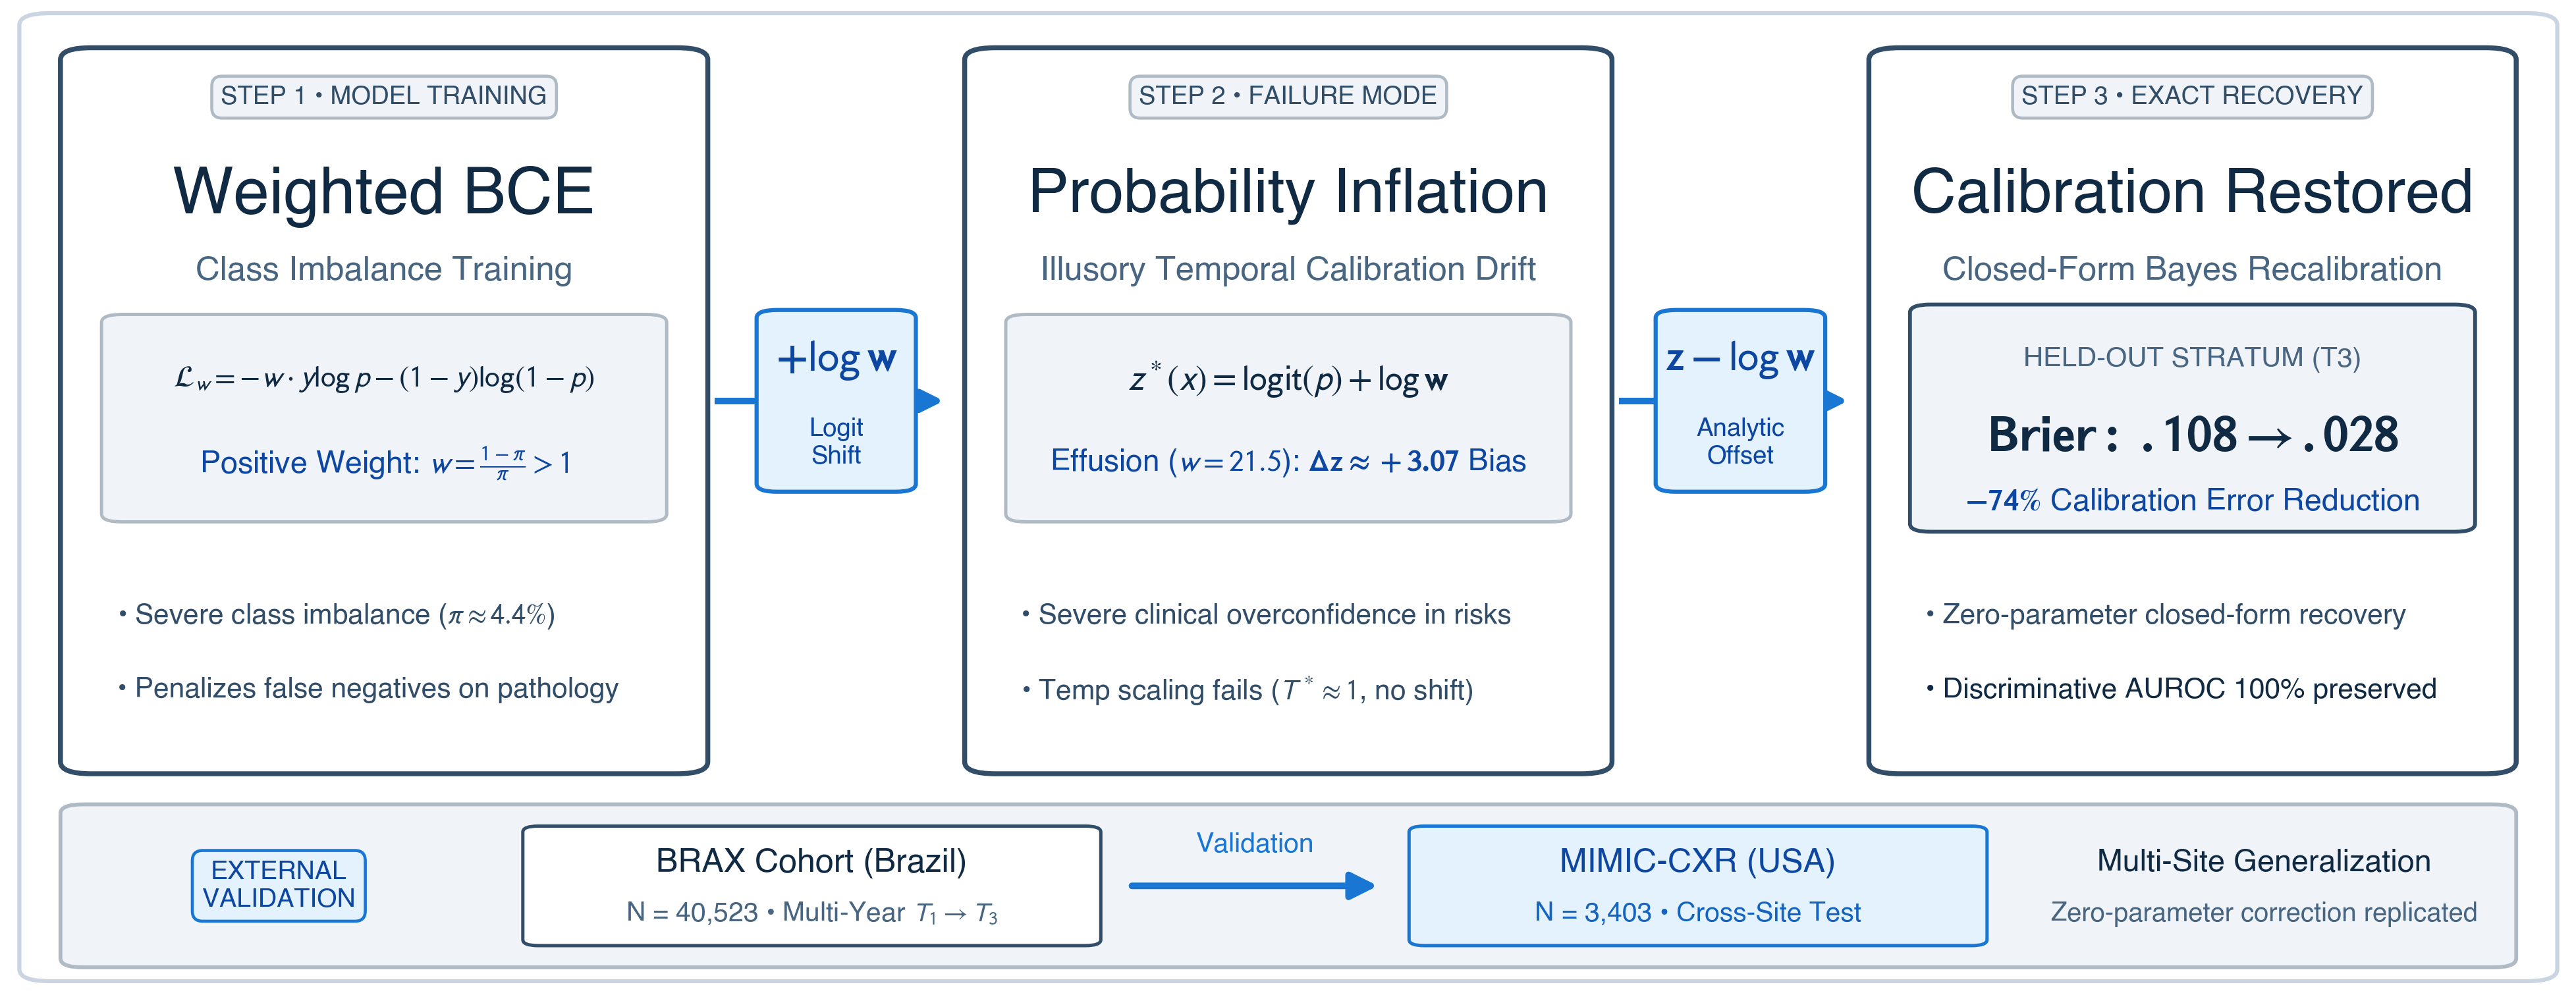
\includegraphics[width=\textwidth]{graphical_abstract.png}
\vspace*{\fill}
\end{graphicalabstract}

\end{frontmatter}

\linenumbers

\section{Introduction}
Deep learning models for chest radiograph interpretation have achieved high discriminatory performance across common thoracic abnormalities~\cite{rajpurkar2017chexnet, reis2022brax}. However, transferring models from stationary retrospective validation to longitudinal clinical deployment introduces substantial distribution shifts as patient populations, imaging protocols, and disease prevalence evolve over time~\cite{finlayson2021clinician, kore2024empirical, shenouda2023assessment}.

While discriminatory ranking (AUROC) often exhibits gradual longitudinal attenuation, high-stakes medical decision support relies fundamentally on \textit{calibrated posterior probabilities}: $P(Y = 1 \mid X = x)$~\cite{vancalster2019calibration, steyerberg2010assessing}. Miscalibrated probabilities distort clinical decision cutoffs, degrade expected utility formulations, and compromise automated triage. Recent studies have reported rapid ``temporal calibration decay,'' asserting that frozen neural networks suffer progressive miscalibration over deployment periods~\cite{guo2022evaluation, hinson2022multisite}. Concurrently, because thoracic datasets exhibit extreme class imbalance (prevalence often $<5\%$), models are routinely trained using positive-weighted binary cross-entropy (BCE)~\cite{rajpurkar2017chexnet, buda2018systematic}.

In this work, we demonstrate that these two phenomena are deeply entangled: the prevailing attribution of temporal calibration collapse to intrinsic feature drift is largely an artifact of uncorrected post-training calibration offsets under label distribution shifts~\cite{alexandari2020maximum, davis2020detection}. Under population risk minimization, training with positive loss weight $w > 1$ mathematically shifts the Bayes-optimal logit by an additive constant $+\ln w$~\cite{king2001logistic, caplin2022calibrating}. Standard post-hoc calibration methods---most notably temperature scaling~\cite{guo2017calibration}---rescale logit variance ($z / T$) but cannot adjust the logit intercept. Consequently, weighted models continuously over-predict positive probabilities, producing severe Brier score and Expected Calibration Error (ECE) degradation that compounds as disease prevalence fluctuates over time.

\subsection{Related Work}
\textbf{Probability Calibration and Class Imbalance:} Deep neural networks frequently exhibit over-confidence due to unconstrained cross-entropy minimization~\cite{guo2017calibration}. While post-hoc recalibration techniques such as temperature scaling, histogram binning, and Platt scaling are standard~\cite{guo2017calibration, platt1999probabilistic, vancalster2019calibration}, they were primarily formulated for balanced distributions. In clinical prediction modeling, Piccininni et al.~\cite{piccininni2024understanding} demonstrated that correcting class imbalance via resampling inherently distorts probability calibration, while plug-in corrections can recover valid absolute risks. In loss-based weighting, King and Zeng~\cite{king2001logistic} established in classical logistic regression that choice-based sampling proportion adjustments induce an intercept shift of $\ln w$. Recently, Caplin, Martin, and Marx~\cite{caplin2022calibrating} analyzed loss-weighted deep learning through an economic lens, proving that class weighting is mathematically incompatible with raw posterior calibration and formulating an inverse machine learning framework to recover undistorted likelihoods on a static pneumonia task. However, their work was confined to single-split evaluations, leaving unexamined how loss-induced logit shifts behave under sequential temporal cohort shifts, whether standard temperature scaling fails, and how post-hoc recalibration performs under cross-institutional transfer.

\textbf{Distribution Shift and Selective Prediction:} Temporal dataset shift encompasses changes in feature distributions $P(X)$, conditional distributions $P(Y \mid X)$, and label priors $P(Y)$~\cite{finlayson2021clinician, davis2020detection}. Alexandari et al.~\cite{alexandari2020maximum} established that bias-corrected calibration provides robust adaptation under label shift. Selective classification allows models to abstain on ambiguous inputs and route them to expert radiologists~\cite{geifman2017selective, kompa2021second, aperstein2026knowing}. While selective triage studies focus primarily on abstention policies, the interaction between loss-induced calibration distortion and downstream referral triage remains unexplored. In this work, we employ selective prediction as an operational lens to examine the real-world clinical trade-offs between calibrated probability estimation and screening triage.

\subsection{Contributions}
To resolve algorithmic loss bias from distribution shift across cohort strata, this paper provides:
\begin{enumerate}
    \item \textbf{Controlled $2 \times 2$ Experimental Design:} We evaluate two clinical architectures (DenseNet-121, ResNet-50) and two loss objectives (standard vs. positive-weighted BCE) across three independent seeds (12 models total) on 40,523 radiographs from BRAX~\cite{reis2022brax}, tracking discrimination and calibration across three held-out deidentified-date strata ($T_1, T_2, T_3$) with strict patient isolation.
    \item \textbf{Mathematical Derivation and Empirical Clustering of Logit Shift:} We prove that positive-weighted BCE introduces a constant population logit offset $\ln w$ (Section S1 of the Supplementary Material). Across 16,604 evaluations, finite neural network logits cluster tightly around theoretical $\ln w$ (mean $\Delta z = 3.29 \pm 0.81$ vs. theoretical $3.07$ for Pleural Effusion). Crucially, we prove that temperature scaling structurally fails to correct this intercept displacement ($\alpha \approx -2.96$), whereas a closed-form analytic offset ($z - \ln w$) eliminates 73.7\% of stratum $T_3$ Brier error ($0.1079 \to 0.0284$) and restores calibration parity without model retraining.
    \item \textbf{Leak-Free Cross-Fitting and Patient-Clustered Bootstrap:} We implement a 5-fold patient-clustered cross-fitting protocol on $T_1$ and evaluate out-of-sample generalization on $T_2$ and $T_3$ backed by 2,000-replicate patient-clustered bootstrap intervals.
    \item \textbf{Operational Selective Prediction and Cross-Institutional Transportability:} We formalize budget-constrained uncertainty-ranked selective deferral, quantifying the trade-off between calibrated risk estimation and screening triage. We stress-test external transportability on MIMIC-CXR-JPG (3,403 images, 289 patients), delineating the capabilities and boundaries of zero-retraining recalibration under real-world domain shift.
\end{enumerate}

\section{Materials and Methods}

\subsection{Dataset and Cohort Stratification}
We utilize the Brazilian Chest X-ray (BRAX) v1.1.0 benchmark~\cite{reis2022brax}. BRAX contains 40,967 radiographs labeled with 14 thoracic findings extracted from Portuguese reports via a validated NLP pipeline. After excluding 444 radiographs from 89 patients whose examinations crossed partition boundaries, the analytic cohort comprised 40,523 radiographs acquired at Hospital Israelita Albert Einstein in S\~ao Paulo, Brazil.

In compliance with HIPAA de-identification standards, timestamps are protected as fictitious 8-digit calendar integers (\texttt{YYYYMMDD}) preserving intra-patient acquisition intervals. Because cross-patient calendar synchronization is unverified, partitions represent sequential deidentified-date strata rather than synchronized calendar years. Studies are partitioned chronologically around a strict model freeze boundary ($T_{\text{freeze}} = \text{2015-07-01}$): training studies before 2013-09-01 ($N = 25,123$ images, 11,265 patients, 14,315 studies); validation studies between 2013-09-01 and 2015-06-30 ($N = 7,098$ images, 3,281 patients, 4,012 studies); and held-out test studies between 2015-07-01 and 2017-12-17 ($N = 8,302$ images, 3,807 patients, 4,670 studies) partitioned into three consecutive strata: $T_1$ ($N=1,879$), $T_2$ ($N=3,987$), and $T_3$ ($N=2,436$). Strict patient isolation is enforced ($\text{Patients}_{\text{train}} \cap \text{Patients}_{\text{val}} \cap \text{Patients}_{\text{test}} = \emptyset$). Complete cohort characteristics are summarized in Table~\ref{tab:cohort_demographics}.

\begin{table*}[!t]
\caption{Cohort Demographics, Radiographic Projections, and Target Condition Prevalence across Stratified Cohorts}
\label{tab:cohort_demographics}
\centering
\resizebox{\textwidth}{!}{%
\begin{tabular}{lllllllllll}
\toprule
Cohort Stratum & Images (N) & Patients (N) & Studies (N) & Sex (\% M / F) & Age (Mean ± SD) & Views (\% PA / AP / Lat / Unk) & Pleural Effusion N (\%) & Cardiomegaly N (\%) & Pneumonia N (\%) & Edema N (\%) \\
\midrule
Train (Pre-deployment) & 25,123 & 11,265 & 14,315 & 49.3\% / 50.7\% & 46.0 ± 24.3 & 34.0\% / 13.5\% / 0.0\% / 27.2\% & 1,116 (4.44\%) & 2,398 (9.55\%) & 456 (1.82\%) & 23 (0.09\%) \\
Val (Pre-deployment) & 7,098 & 3,281 & 4,012 & 49.8\% / 50.2\% & 46.2 ± 24.1 & 34.7\% / 12.2\% / 0.0\% / 27.7\% & 295 (4.16\%) & 681 (9.59\%) & 128 (1.80\%) & 8 (0.11\%) \\
Test T1 (2015) & 1,879 & 913 & 1,039 & 47.8\% / 52.2\% & 44.5 ± 23.9 & 34.4\% / 10.2\% / 0.0\% / 29.0\% & 99 (5.27\%) & 147 (7.82\%) & 50 (2.66\%) & 4 (0.21\%) \\
Test T2 (2016) & 3,987 & 1,832 & 2,249 & 48.5\% / 51.5\% & 46.1 ± 23.8 & 34.6\% / 12.0\% / 0.0\% / 27.6\% & 177 (4.44\%) & 422 (10.58\%) & 79 (1.98\%) & 13 (0.33\%) \\
Test T3 (2017) & 2,436 & 1,164 & 1,382 & 50.9\% / 49.1\% & 46.0 ± 24.6 & 34.4\% / 12.4\% / 0.0\% / 28.1\% & 85 (3.49\%) & 258 (10.59\%) & 50 (2.05\%) & 0 (0.00\%) \\
Test All (Pooled) & 8,302 & 3,807 & 4,670 & 49.0\% / 51.0\% & 45.7 ± 24.1 & 34.5\% / 11.7\% / 0.0\% / 28.1\% & 361 (4.35\%) & 827 (9.96\%) & 179 (2.16\%) & 17 (0.20\%) \\
\bottomrule
\end{tabular}

}
\end{table*}

\subsection{External Stress-Testing Cohort (MIMIC-CXR-JPG)}
To assess whether the mathematical calibration mechanism survives cross-institutional domain shift, frozen BRAX models were externally evaluated on all eligible frontal radiographs (AP and PA views) from the official patient-partitioned MIMIC-CXR-JPG test split~\cite{johnson2019mimic,johnson2019mimicjpg}. The cohort comprises $N = 3,403$ frontal radiographs ($N = 3,041$ diagnostic studies across $N = 289$ unique patients; AP: $2,405$ [$70.67\%$], PA: $998$ [$29.33\%$]). Ground-truth labels were extracted using the official CheXpert labeler under the uncertainty-zero ($U\text{-zero}$) policy: Pleural Effusion $32.18\%$ ($N = 1,095$ positive radiographs across $178$ positive and $273$ negative patients; $990$ studies), Cardiomegaly $26.33\%$ ($N = 896$ across $183$ positive and $282$ negative patients; $808$ studies), Edema $21.33\%$ ($N = 726$ across $150$ positive and $287$ negative patients; $659$ studies), and Pneumonia $10.05\%$ ($N = 342$ across $137$ positive and $286$ negative patients; $309$ studies). Patient-clustered non-parametric bootstrap inference ($B=1,000$ replicates) accounts for repeated within-patient examinations and longitudinal disease transitions across serial studies. No model fine-tuning or retraining was performed.

\subsection{Architectures and Training Objectives}
We evaluate two standard clinical vision architectures initialized from ImageNet pre-trained weights:
\begin{itemize}
    \item \textbf{DenseNet-121}~\cite{densenet2017huang}: Employs dense feature concatenation, standard for thoracic pathology benchmarks~\cite{rajpurkar2017chexnet}.
    \item \textbf{ResNet-50}~\cite{resnet2016he}: Employs residual skip connections as an independent structural comparator.
\end{itemize}

Each architecture is trained under two distinct loss objectives:
\begin{enumerate}
    \item \textbf{Unweighted Binary Cross-Entropy (Standard BCE):}
    \begin{equation}
    \mathcal{L}_{\text{std}}(y, \hat{p}) = - [y \log \hat{p} + (1 - y) \log(1 - \hat{p})]
    \end{equation}
    where $\hat{p} = \sigma(z) = 1 / (1 + e^{-z})$ is the sigmoid probability from raw logit $z$.
    \item \textbf{Positive-Weighted Binary Cross-Entropy (Weighted BCE):}
    \begin{equation}
    \mathcal{L}_{\text{pos}}(y, \hat{p}) = - [w \cdot y \log \hat{p} + (1 - y) \log(1 - \hat{p})]
    \end{equation}
    where $w = (N_{\text{total}} - N_{\text{pos}}) / N_{\text{pos}}$ represents the inverse positive prevalence in the training set (e.g., $w = 21.51$ for Pleural Effusion, $w = 9.48$ for Cardiomegaly, $w = 54.09$ for Pneumonia).
\end{enumerate}

Models are trained with the AdamW optimizer (learning rate $10^{-4}$, weight decay $10^{-2}$) and a Cosine Annealing schedule over 15 epochs (batch size 64, AMP fp16, $512 \times 512$ resolution). Pleural Effusion was pre-specified as the primary target pathology due to its stable evaluability across all longitudinal held-out strata ($T_1=1,879, T_2=3,987, T_3=2,436$); Cardiomegaly, Pneumonia, and Edema served as secondary mechanistic validation targets. Checkpoints were selected by highest validation AUROC. Three random seeds ($S \in \{42, 123, 2026\}$) were trained per configuration (12 models total). For unified benchmarking, a 3-seed probability ensemble was constructed by averaging predicted probabilities: $\bar{p}_{\text{raw}}(x) = \frac{1}{3}\sum_{s \in S} \sigma(z_s(x))$ and $\bar{p}_{\text{corrected}}(x) = \frac{1}{3}\sum_{s \in S} \sigma(z_s(x) - \ln w)$. The empirical logit offset was evaluated across all 16,604 ensemble-paired evaluations ($8,302$ images $\times$ $2$ architectures; $49,812$ seed-level pairs):
\begin{equation}
\Delta z(x) = \bar{z}_w(x) - \bar{z}_u(x) = \frac{1}{3}\sum_{s \in S} \left( z_{w, s}(x) - z_{u, s}(x) \right)
\label{eq:delta_z_definition}
\end{equation}

\subsection{Mathematical Mechanics of Loss Weighting and Calibration}
Under positive-weighted binary cross-entropy, the conditional expected risk with positive weight $w > 0$ is:
\begin{equation}
\mathbb{E}_{Y \mid X} [\mathcal{L}_{\text{pos}}(Y, \hat{p})] = - w \cdot P(Y=1 \mid X) \ln \hat{p} - P(Y=0 \mid X) \ln(1 - \hat{p})
\end{equation}
Setting the first-order condition $\frac{\partial}{\partial z} \mathbb{E}[\mathcal{L}_{\text{pos}}] = 0$ yields the optimal predicted probability:
\begin{equation}
\hat{p}^*(x) = \frac{w \cdot P(Y=1 \mid X=x)}{w \cdot P(Y=1 \mid X=x) + P(Y=0 \mid X=x)}
\end{equation}
Converting to log-odds yields the Bayes-optimal logit:
\begin{equation}
z^*(x) = \ln\left(\frac{P(Y=1 \mid X=x)}{P(Y=0 \mid X=x)}\right) + \ln w = z_{\text{true}}(x) + \ln w
\label{eq:bayes_logit}
\end{equation}
(see Section S1 of the Supplementary Material for the complete algebraic proof). Equation~(\ref{eq:bayes_logit}) derives that positive loss weighting shifts the model's population Bayes-optimal logit by $+\ln w$, connecting classical choice-based sampling corrections~\cite{king2001logistic} with the class-weight likelihood recovery formulation of Caplin et al.~\cite{caplin2022calibrating}. In finite neural networks, empirical logits fluctuate around this theoretical attractor.

\subsubsection{Limitation of Temperature Scaling}
Temperature scaling~\cite{guo2017calibration} adjusts probabilities via a single scalar $T$: $p_{\text{temp}} = \sigma(z / T)$. In the Cox calibration framework~\cite{vancalster2019calibration, steyerberg2010assessing}:
\begin{equation}
\text{logit}(P(Y = 1 \mid X)) = \alpha + \beta \cdot \text{logit}(\hat{p})
\label{eq:cox_calibration}
\end{equation}
where $\alpha = 0$ represents perfect calibration-in-the-large and $\beta = 1$ denotes ideal slope. Because positive weighting induces an additive shift $z \approx z_{\text{true}} + \ln w$, the uncorrected logit suffers an acute intercept discrepancy ($\alpha \approx -\ln w \ll 0$). Temperature scaling multiplies logits by $1/T$, adjusting slope $\beta \to \beta \cdot T$, but is mathematically incapable of adjusting the additive constant $\alpha$. In low-prevalence clinical domains where negative cases dominate, the optimizer is constrained by conflicting slope and intercept pressures, typically selecting $T^* \approx 1.0$ without resolving the underlying intercept displacement.

\subsubsection{Post-Hoc Recalibration Suite and Computational Complexity}
We evaluate four post-hoc recalibration functions:
\begin{enumerate}
    \item \textbf{Temperature Scaling ($T^*$):} $p = \sigma(z / T^*)$, optimized via bounded Brent minimization on $[0.01, 50.0]$ with an explicit monotonicity constraint; incurs $O(N_{\mathrm{val}})$ optimization and $O(1)$ inference.
    \item \textbf{Analytic Offset ($z - \ln w$):} Directly subtracts the theoretical logit shift: $p = \sigma(z - \ln w)$. Requires zero validation data and zero numerical optimization ($O(1)$ training and inference), resetting $\alpha \approx 0$ by construction while preserving model discrimination and slope.
    \item \textbf{Fitted Offset ($z + a^*$):} Optimizes a scalar intercept $a^* \in [-10.0, 10.0]$ on validation log-likelihood, holding slope fixed at $1.0$ ($O(N_{\mathrm{val}})$ fitting, $O(1)$ inference).
    \item \textbf{Platt Scaling ($a + bz$):} Logistic regression on logits with a non-negative slope constraint ($b \ge 0$) ($O(k \cdot N_{\mathrm{val}})$ fitting, $O(1)$ inference).
\end{enumerate}

\subsection{Cross-Fitting and Resampling Evaluation Protocol}
On deployment stratum $T_1$ (2015-H2), calibrator parameters are estimated using \textbf{5-fold patient-clustered cross-fitting} (all studies from any given patient assigned to a single fold). Calibrators fit on $T_1$ are frozen and applied strictly out-of-sample on later strata $T_2$ (2016) and $T_3$ (2017). All 95\% confidence intervals are computed using $B = 2,000$ patient-clustered bootstrap resamples with replacement ($B = 1,000$ for external MIMIC validation). Paired calibrator contrasts are evaluated on identical bootstrap resamples.

\subsection{Selective Prediction and Deferral Policy}
In operational deployment, models can selectively defer ambiguous examinations to expert radiologists~\cite{geifman2017selective, kompa2021second, aperstein2026knowing}. Rather than developing novel rejection algorithms, our selective prediction formulation evaluates how loss weighting and calibration impact clinical referral efficiency and automated error rates.

Operating decision cutoffs $t^*$ are determined strictly on development stratum $T_1$ using Youden's $J$ index ($t^* \approx 0.014$ for unweighted, $t^* \approx 0.022$ for analytic offset, $t^* \approx 0.33$ for raw weighted models). We define a threshold-relative uncertainty metric based on piecewise distance from $t^*$:
\begin{equation}
u(x) = 1 - \frac{|\hat{p}(x) - t^*|}{\mathbb{I}(\hat{p}(x) \ge t^*)(1 - t^*) + \mathbb{I}(\hat{p}(x) < t^*)t^*} \in [0, 1]
\label{eq:uncertainty}
\end{equation}
where $u(x) \to 1$ indicates maximal ambiguity ($\hat{p}(x) \approx t^*$) and $u(x) \to 0$ indicates decisive confidence. At coverage budget $C \in [0.5, 1.0]$, the system retains the fraction $C$ of cases with lowest uncertainty ($N_{\text{auto}} = \lceil C \cdot N \rceil$) and refers the remaining $1 - C$ to radiologist review ($N_{\text{ref}} = N - N_{\text{auto}}$).

We track triage outcomes across five distinct metrics: (i) retained positives ($N_{\text{pos, ret}}$); (ii) automated true positives ($TP_{\text{auto}} = \sum_{i \in \text{Auto}} \mathbb{I}(y_i = 1 \land \hat{y}_i = 1)$); (iii) automated false negatives ($FN_{\text{auto}} = \sum_{i \in \text{Auto}} \mathbb{I}(y_i = 1 \land \hat{y}_i = 0)$, where $TP_{\text{auto}} + FN_{\text{auto}} = N_{\text{pos, ret}}$); (iv) retained sensitivity ($\text{Sens}_{\text{ret}} = TP_{\text{auto}} / N_{\text{pos, ret}}$); and (v) full-cohort triage sensitivity ($\text{Sens}_{\text{triage}} = 1 - FN_{\text{auto}} / N_{\text{pos, total}}$), assuming deferred cases are correctly diagnosed by expert radiologists.

\begin{algorithm}[!t]
\caption{Budget-Constrained Uncertainty-Ranked Selective Deferral Pipeline}
\label{alg:selective_deferral}
\begin{algorithmic}[1]
\REQUIRE Cohort radiographs $\{x_i\}_{i=1}^N$, trained neural network $f_\theta$, positive loss weight $w$, clinical operating threshold $t^*$, target coverage budget $C \in (0, 1]$.
\ENSURE Automated decisions $\{\hat{y}_i : i \in \mathcal{S}\}$ and referred examination set $\mathcal{D}$.
\STATE \textbf{Phase 1: Analytic Recalibration and Uncertainty Scoring}
\FOR{$i = 1$ \TO $N$}
    \STATE Compute raw network logit: $z_i \leftarrow f_\theta(x_i)$
    \IF{model was trained with positive class weight $w > 1$}
        \STATE Apply constant-time closed-form offset: $\tilde{z}_i \leftarrow z_i - \ln(w)$
    \ELSE
        \STATE $\tilde{z}_i \leftarrow z_i$
    \ENDIF
    \STATE Compute calibrated probability: $\hat{p}_i \leftarrow \sigma(\tilde{z}_i) = \frac{1}{1 + \exp(-\tilde{z}_i)}$
    \STATE Compute threshold-relative normalizer:
    \STATE \quad $s_i \leftarrow \begin{cases} 1 - t^*, & \text{if } \hat{p}_i \ge t^* \\ t^*, & \text{otherwise} \end{cases}$
    \STATE Compute normalized threshold-proximity uncertainty:
    \STATE \quad $u_i \leftarrow 1 - \min\left(1, \frac{|\hat{p}_i - t^*|}{s_i}\right) \in [0, 1]$
\ENDFOR
\STATE \textbf{Phase 2: Budget-Constrained Triage Partitioning}
\STATE Compute automation quota: $k \leftarrow \min\left(N, \max\left(1, \lceil C \cdot N \rceil\right)\right)$
\STATE Sort cohort indices by ascending uncertainty: $\pi \leftarrow \text{argsort}(\{u_1, \dots, u_N\})$
\STATE Partition cohort into automated and deferred sets:
\STATE \quad $\mathcal{S} \leftarrow \{\pi(1), \pi(2), \dots, \pi(k)\} \quad$ \COMMENT{Retained automated cohort}
\STATE \quad $\mathcal{D} \leftarrow \{\pi(k+1), \dots, \pi(N)\} \quad$ \COMMENT{Referred to expert radiologist review}
\STATE \textbf{Phase 3: Decision Assignment}
\FOR{$i \in \mathcal{S}$}
    \STATE Assign automated binary classification: $\hat{y}_i \leftarrow \mathbb{I}(\hat{p}_i \ge t^*)$
\ENDFOR
\RETURN Automated decisions $\{\hat{y}_i\}_{i \in \mathcal{S}}$, deferred cases $\mathcal{D}$.
\end{algorithmic}
\end{algorithm}

\begin{figure*}[!t]
\centering
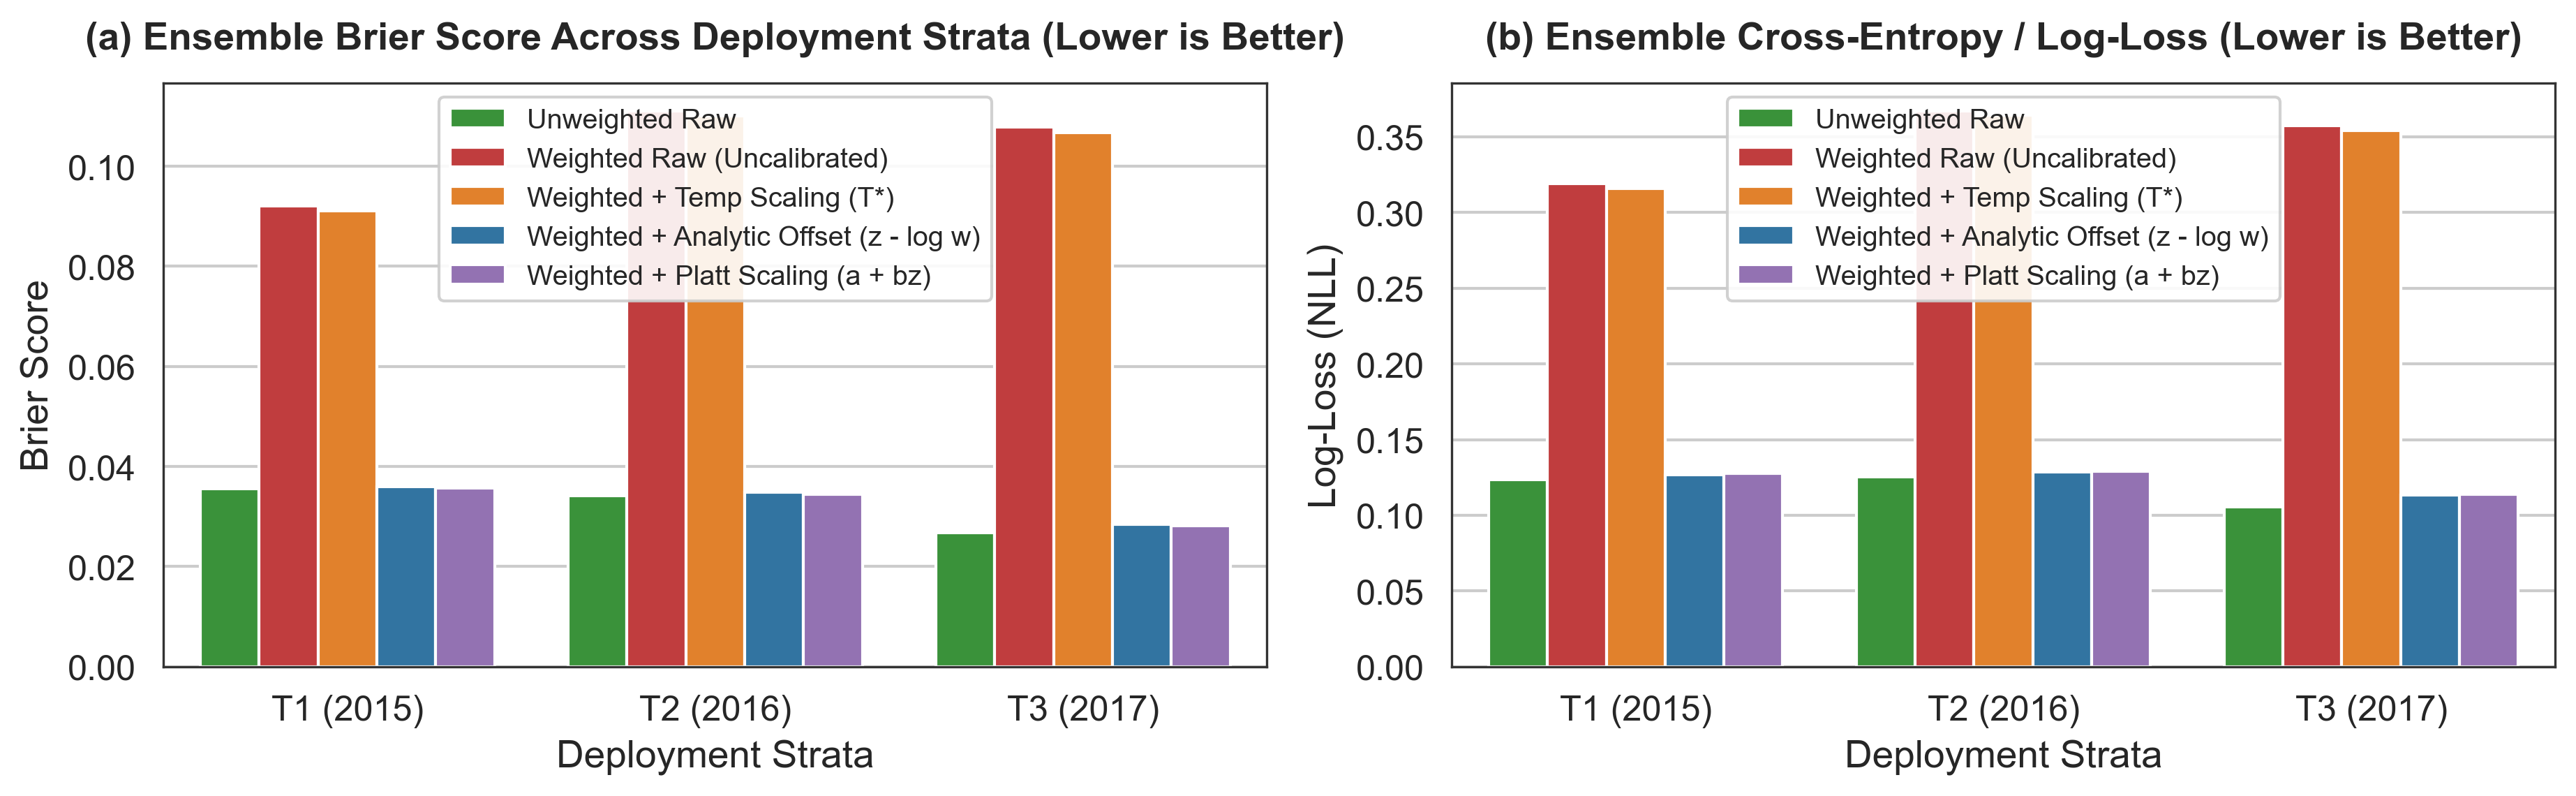
\includegraphics[width=0.85\textwidth]{figures/fig3_recalibration_comparison.png}
\caption{Multi-calibrator evaluation on Pleural Effusion for the DenseNet-121 3-seed ensemble across sequential deidentified-date strata ($T_1, T_2, T_3$), directly visualizing Table~\ref{tab:calibrator_comparison}. (a) Brier score and (b) Log-loss. Temperature scaling fails to reduce probability error in weighted models, whereas Analytic Offset ($z - \log w$) and Platt Scaling reduce Brier score by 73.7\% ($\Delta\text{Brier} = -0.0795$), matching unweighted models.}
\label{fig:calibrator_comparison}
\end{figure*}

\section{Experimental Results}

\subsection{Experimental Matrix: Discrimination vs. Calibration Trajectories}
Table~\ref{tab:factorial_matrix} presents the comprehensive evaluation of the $2 \times 2$ experimental design comprising two architectures and two loss objectives (with three independently trained random seed replications per configuration, 12 models total) for Pleural Effusion, Cardiomegaly, and Pneumonia across chronological strata $T_1, T_2, T_3$.

\subsubsection{Discrimination Attenuation vs. Calibration Trajectories}
Both architectures exhibit moderate discriminatory attenuation across subsequent deidentified-date cohort strata. For DenseNet-121 on Pleural Effusion, AUROC decreases from $0.9335 \pm 0.0052$ at $T_1$ to $0.8731 \pm 0.0120$ at $T_3$ ($\Delta\text{AUROC} = -0.0604$); ResNet-50 exhibits an identical downward trajectory ($0.9295 \pm 0.0113 \to 0.8608 \pm 0.0190$, $\Delta\text{AUROC} = -0.0687$; Table~\ref{tab:factorial_matrix}). This confirms that discriminatory attenuation occurs gradually across subsequent cohort strata regardless of loss objective.

In stark contrast, probability calibration diverges sharply by loss objective. For unweighted models, Brier scores are low and actually improve as prevalence falls ($0.0369 \pm 0.0029 \to 0.0279 \pm 0.0009$ on Pleural Effusion). For positive-weighted models, Brier scores are severely elevated and appear to deteriorate over time ($0.1081 \pm 0.0394 \to 0.1254 \pm 0.0456$ on DenseNet-121; $0.1256 \pm 0.0325 \to 0.1392 \pm 0.0310$ on ResNet-50), with ECE exceeding 22\%. Tracking the excess penalty $\Delta\text{Brier} = \text{Brier}_{\text{weighted}} - \text{Brier}_{\text{unweighted}}$ across sequential strata reveals the operational mechanism: when prevalence declines (Pleural Effusion: $5.27\% \to 3.49\%$), the excess penalty expands ($+0.0712 \to +0.0975$); when prevalence rises (Cardiomegaly: $7.82\% \to 10.59\%$), it attenuates ($+0.0729 \to +0.0683$); and when prevalence is steady (Pneumonia: $2.66\% \to 2.05\%$), it remains fixed ($+0.1079 \to +0.1112$). A static training logit shift produces surplus false-positive probability mass that is penalized more severely when deployment disease prevalence drops, expanding the apparent temporal calibration gap.

\begin{table*}[!t]
\caption{Experimental Matrix Evaluation: Primary Longitudinal Performance across Architectures, Loss Objectives, and Thoracic Pathologies (Strata $T_1 \to T_3$). Values represent mean $\pm$ standard deviation across three independently trained random seeds ($S \in \{42, 123, 2026\}$). Complete 17-column trajectories across all intermediate deployment strata ($T_1, T_2, T_3$) and log-loss metrics are detailed in Supplementary Table~S3.}
\label{tab:factorial_matrix}
\centering
\small
\resizebox{\textwidth}{!}{%
\begin{tabular}{lllccccc}
\toprule
\textbf{Architecture} & \textbf{Objective} & \textbf{Pathology} & \textbf{AUROC ($T_1 \to T_3$)} & \textbf{$\Delta\text{AUROC}$} & \textbf{Brier ($T_1 \to T_3$)} & \textbf{$\Delta\text{Brier}$} & \textbf{ECE $T_3$} \\
\midrule
DenseNet-121 & Unweighted BCE & Pleural Effusion & 0.934 $\to$ 0.873 & -0.060 & 0.037 $\to$ 0.028 & -0.009 & 0.0090 \\
DenseNet-121 & Unweighted BCE & Cardiomegaly & 0.908 $\to$ 0.902 & -0.006 & 0.053 $\to$ 0.068 & +0.015 & 0.0210 \\
DenseNet-121 & Unweighted BCE & Pneumonia & 0.847 $\to$ 0.865 & +0.017 & 0.024 $\to$ 0.019 & -0.005 & 0.0095 \\
DenseNet-121 & Unweighted BCE & Edema* & 0.540 $\to$ -- & -- & 0.002 $\to$ 0.000 & -0.002 & 0.0029 \\
\midrule
DenseNet-121 & Pos-Weighted BCE & Pleural Effusion & 0.906 $\to$ 0.839 & -0.067 & 0.108 $\to$ 0.125 & +0.017 & 0.2227 \\
DenseNet-121 & Pos-Weighted BCE & Cardiomegaly & 0.874 $\to$ 0.858 & -0.016 & 0.126 $\to$ 0.136 & +0.010 & 0.1969 \\
DenseNet-121 & Pos-Weighted BCE & Pneumonia & 0.818 $\to$ 0.842 & +0.024 & 0.131 $\to$ 0.130 & -0.002 & 0.2425 \\
DenseNet-121 & Pos-Weighted BCE & Edema* & 0.612 $\to$ -- & -- & 0.061 $\to$ 0.064 & +0.002 & 0.1274 \\
\midrule
ResNet-50 & Unweighted BCE & Pleural Effusion & 0.930 $\to$ 0.861 & -0.069 & 0.037 $\to$ 0.028 & -0.009 & 0.0132 \\
ResNet-50 & Unweighted BCE & Cardiomegaly & 0.890 $\to$ 0.879 & -0.011 & 0.057 $\to$ 0.071 & +0.014 & 0.0175 \\
ResNet-50 & Unweighted BCE & Pneumonia & 0.843 $\to$ 0.880 & +0.037 & 0.024 $\to$ 0.019 & -0.005 & 0.0106 \\
ResNet-50 & Unweighted BCE & Edema* & 0.556 $\to$ -- & -- & 0.002 $\to$ 0.000 & -0.002 & 0.0017 \\
\midrule
ResNet-50 & Pos-Weighted BCE & Pleural Effusion & 0.879 $\to$ 0.819 & -0.060 & 0.126 $\to$ 0.139 & +0.014 & 0.2751 \\
ResNet-50 & Pos-Weighted BCE & Cardiomegaly & 0.830 $\to$ 0.799 & -0.031 & 0.142 $\to$ 0.152 & +0.011 & 0.2338 \\
ResNet-50 & Pos-Weighted BCE & Pneumonia & 0.835 $\to$ 0.823 & -0.012 & 0.167 $\to$ 0.169 & +0.002 & 0.3253 \\
ResNet-50 & Pos-Weighted BCE & Edema* & 0.549 $\to$ -- & -- & 0.069 $\to$ 0.075 & +0.005 & 0.1670 \\
\bottomrule
\end{tabular}

}
\end{table*}

\subsection{Multi-Calibrator Comparison}
Table~\ref{tab:calibrator_comparison} and Fig.~\ref{fig:calibrator_comparison} benchmark post-hoc calibrators on Pleural Effusion across 2,000 patient-clustered bootstrap resamples on the 3-seed ensemble.

\begin{table*}[!t]
\caption{Multi-Calibrator Comparison on Pleural Effusion: Deidentified-Date Ensemble Performance, Calibration Intercept ($\alpha$), Slope ($\beta$), and Paired Bootstrap Contrasts. Complete 12-column factorial evaluation across all intermediate strata and log-loss is provided in Supplementary Table~S4.}
\label{tab:calibrator_comparison}
\centering
\small
\resizebox{\textwidth}{!}{%
\begin{tabular}{lllccccc}
\toprule
\textbf{Architecture} & \textbf{Loss Objective} & \textbf{Calibrator} & \textbf{Brier ($T_1 \to T_3$)} & \textbf{$T_3$ $\alpha$} & \textbf{$T_3$ $\beta$} & \textbf{$T_3$ ECE} & \textbf{$T_3\ \Delta\text{Brier}$ vs Raw [95\% CI]} \\
\midrule
DenseNet-121 & Weighted BCE & Raw (Uncalibrated) & 0.092 $\to$ 0.108 & -2.964 & 1.048 & 0.2227 & -- \\
DenseNet-121 & Weighted BCE & Temperature Scaling ($T^*$) & 0.091 $\to$ 0.107 & -2.962 & 1.029 & 0.2190 & -0.0011 [-0.0014, -0.0009] \\
DenseNet-121 & Weighted BCE & Analytic Offset ($z - \log w$) & 0.036 $\to$ 0.028 & -0.445 & 0.929 & 0.0126 & \textbf{-0.0795} [-0.0893, -0.0697] \\
DenseNet-121 & Weighted BCE & Platt Scaling ($a + bz$) & 0.036 $\to$ 0.028 & -0.229 & 1.128 & 0.0176 & \textbf{-0.0798} [-0.0894, -0.0702] \\
DenseNet-121 & Unweighted BCE & Raw Baseline & 0.036 $\to$ 0.027 & +0.147 & 1.044 & 0.0040 & -- \\
\midrule
ResNet-50 & Weighted BCE & Raw (Uncalibrated) & 0.110 $\to$ 0.123 & -2.853 & 1.950 & 0.2751 & -- \\
ResNet-50 & Weighted BCE & Temperature Scaling ($T^*$) & 0.088 $\to$ 0.101 & -2.608 & 1.184 & 0.1993 & -0.0220 [-0.0241, -0.0198] \\
ResNet-50 & Weighted BCE & Analytic Offset ($z - \log w$) & 0.040 $\to$ 0.029 & +1.075 & 1.405 & 0.0158 & \textbf{-0.0936} [-0.1022, -0.0844] \\
ResNet-50 & Weighted BCE & Platt Scaling ($a + bz$) & 0.038 $\to$ 0.030 & -0.191 & 1.178 & 0.0223 & \textbf{-0.0930} [-0.1007, -0.0849] \\
ResNet-50 & Unweighted BCE & Raw Baseline & 0.036 $\to$ 0.027 & -0.077 & 1.095 & 0.0109 & -- \\
\bottomrule
\end{tabular}

}
\end{table*}

For weighted DenseNet-121, temperature scaling optimizes $T^* \approx 1.0$, producing an uncalibrated $T_3$ Brier score of $0.1067$ compared to raw $0.1079$ ($\Delta\text{Brier} = -0.0011$ [95\% CI: $-0.0014, -0.0009$]) while leaving the calibration intercept severely displaced ($\alpha = -2.9615$ vs. raw $-2.9638$). For ResNet-50, temperature scaling achieves modest variance shrinkage ($\Delta\text{Brier} = -0.0220$ [$-0.0241, -0.0198$]), but leaves the underlying intercept discrepancy uncorrected ($\alpha = -2.6080$ vs. raw $-2.8526$). Temperature scaling is mathematically incapable of adjusting this intercept displacement.

In contrast, subtracting the theoretical logit offset ($z - \ln w$, with $\ln(21.51) = +3.068$) drops $T_3$ Brier from $0.1079$ to $0.0284$ ($\Delta\text{Brier} = -0.0795$ [95\% CI: $-0.0893, -0.0697$], 73.7\% error reduction), reducing ECE from 22.3\% to 1.26\% and shifting the Cox intercept from $\alpha = -2.9638$ to $-0.4451$ while perfectly preserving the calibration slope ($\beta = 0.9292$). Fitted Offset ($z + a^*$) and Platt Scaling achieve identical performance ($T_3$ Brier: $0.0289$ and $0.0281$; $\Delta\text{Brier} = -0.0790$ and $-0.0798$). For ResNet-50, Analytic Offset similarly eliminates 76.3\% of probability error ($0.1227 \to 0.0291$, $\Delta\text{Brier} = -0.0936$ [95\% CI: $-0.1022, -0.0844$]), confirming that intercept neutralization is architecturally universal.

\subsubsection{\texorpdfstring{Empirical Verification of Logit Offset: $\Delta z \approx \ln w$}{Empirical Verification of Logit Offset: Delta z approx ln w}}
\label{sec:logit_offset}
Evaluating logit differences $\Delta z(x) = \bar{z}_w(x) - \bar{z}_u(x)$ across all 16,604 ensemble evaluations (Fig.~\ref{fig:logit_offset}) confirms that finite neural networks cluster tightly around theoretical $\ln w$: Pleural Effusion ($\ln w = 3.07$) observed mean $\Delta z = 3.29 \pm 0.81$ (median $3.25$); Pneumonia ($\ln w = 3.99$) observed $3.83 \pm 0.74$ (median $3.84$); and Cardiomegaly ($\ln w = 2.25$) observed $2.64 \pm 1.04$ (median $2.60$). For Edema ($w = 1091.3, \ln w = 7.00$), acute training scarcity (23 positive cases) causes optimization saturation, bounding empirical shifts at $\Delta z = 3.69 \pm 1.47$ (median $3.46$) due to $L_2$ regularization. Equal-mass reliability diagrams (Fig.~\ref{fig:reliability}) demonstrate that the analytic offset realigns curves tightly with the ideal diagonal across all strata.

\begin{figure*}[!t]
\centering
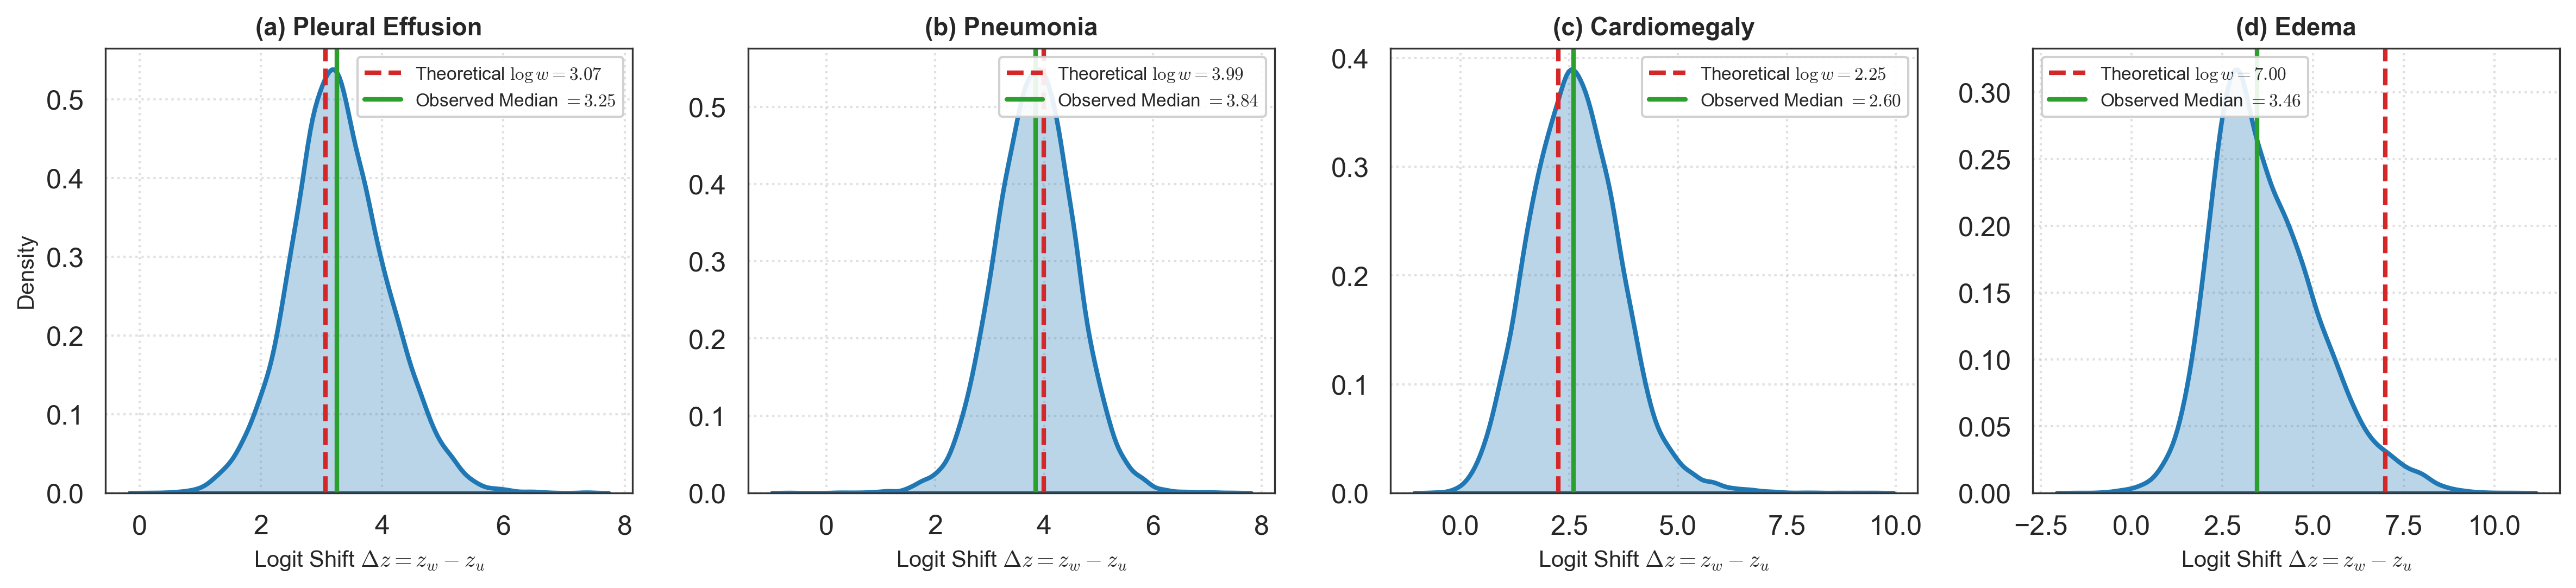
\includegraphics[width=\textwidth]{figures/fig6_logit_offset_verification.png}
\caption{Empirical verification of theoretical logit shift ($z_w - z_u \approx \log w$) across 16,604 held-out deidentified-date image evaluations ($8,302\text{ images} \times 2\text{ architectures}$, with $\Delta z$ computed as the mean difference across the three seed-matched weighted/unweighted model pairs). Kernel density estimates (blue) of observed logit differences between positive-weighted and unweighted models cluster tightly around the theoretical population attractor $\log w$ (dashed red line; observed median in solid green) across Pleural Effusion (a), Pneumonia (b), and Cardiomegaly (c). For Edema (d), extreme training class scarcity ($w > 1000$) induces optimization saturation, bounding empirical shifts near $+3.69$.}
\label{fig:logit_offset}
\end{figure*}

\begin{figure}[!b]
\centering
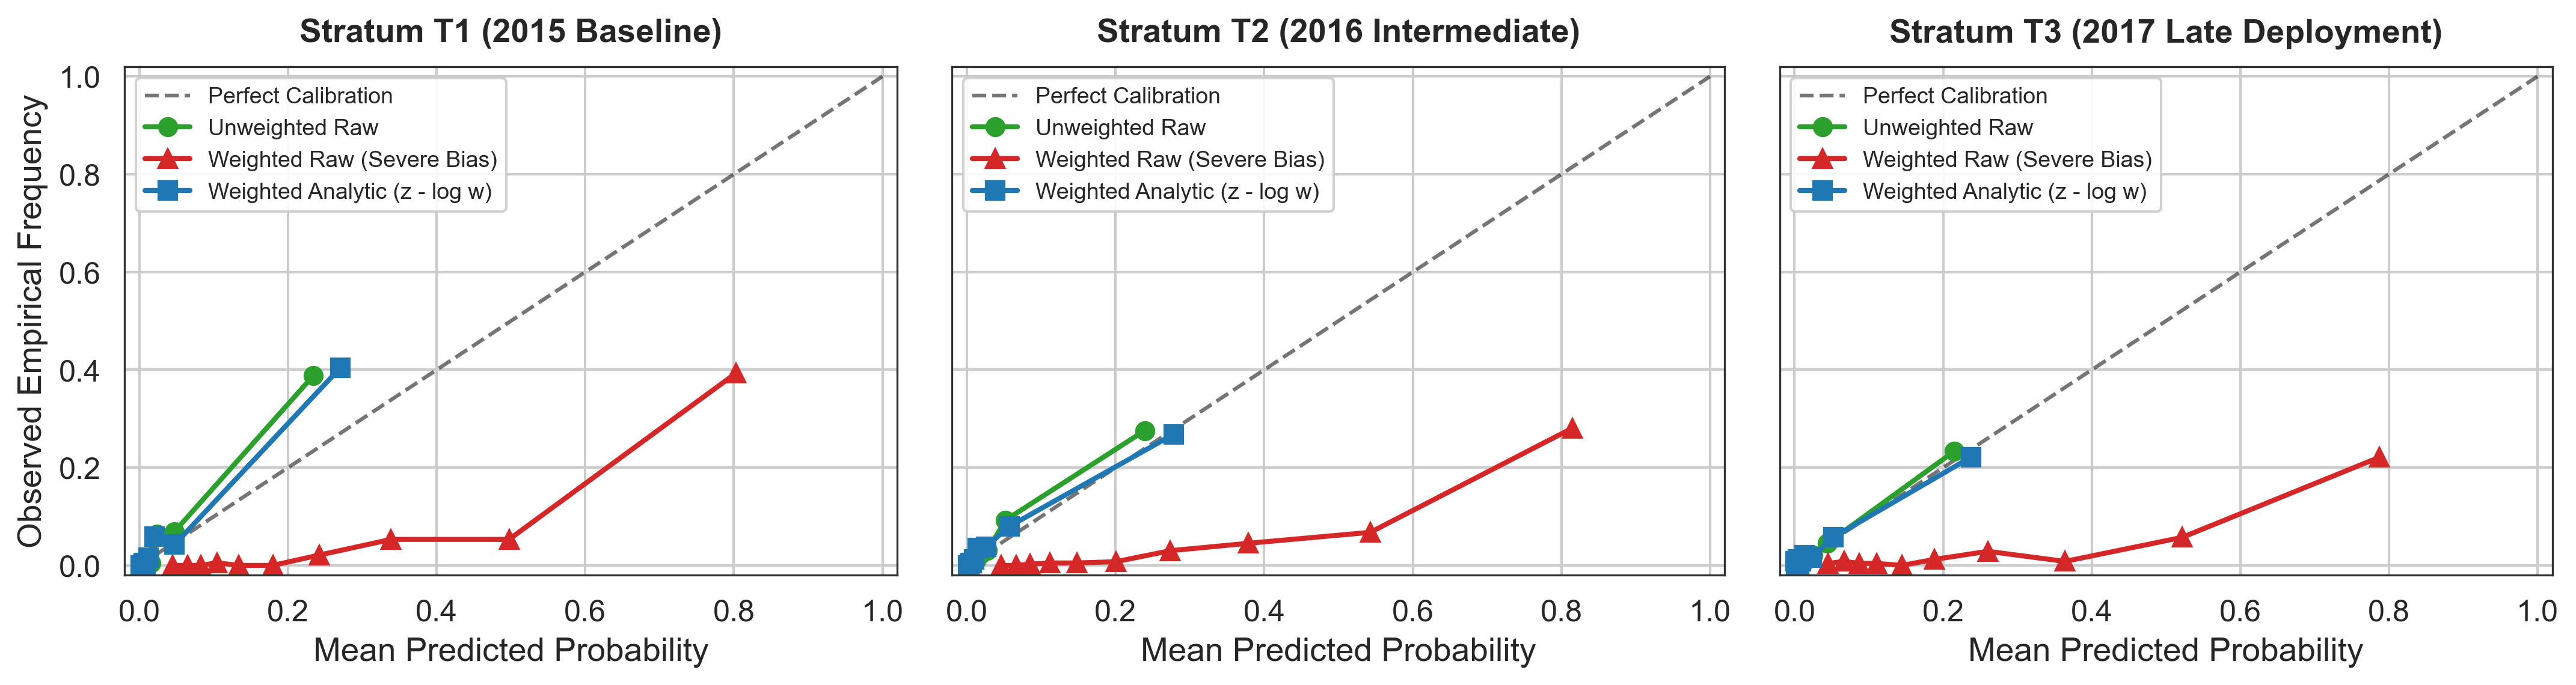
\includegraphics[width=0.75\linewidth]{figures/fig5_reliability_diagrams.png}
\caption{Reliability diagrams for Pleural Effusion (DenseNet-121 3-seed ensemble) across held-out deidentified-date strata ($T_1, T_2, T_3$). Raw weighted models (red) severely over-predict event probabilities across all bins. Analytic offset calibration (blue) and unweighted models (green) remain tightly calibrated to the ideal diagonal across all deployment windows.}
\label{fig:reliability}
\end{figure}

\subsection{Selective Prediction and Workload Triage Simulation}
Table~\ref{tab:selective_prediction} and Fig.~\ref{fig:selective_prediction} summarize the selective triage simulation on later held-out stratum $T_3$ ($N = 2,436$ radiographs, 85 positive Pleural Effusion cases) under development thresholds. At 100\% coverage (full automation), the raw weighted model incurs 16.0 missed cases ($FN_{\text{auto}}$) with Brier 0.1079. Calibrated Analytic Offset under matched threshold ($t^* \approx 0.022$) yields identical sensitivity (81.18\%) and 16.0 missed cases, but with an almost four-fold lower Brier score of 0.0284. Unweighted raw models achieve 12.0 missed cases (sensitivity 85.88\%, Brier 0.0268).

\begin{table*}[!t]
\caption{Selective Prediction and Reader Referral Triage Simulation on Later Held-Out Stratum $T_3$ ($N = 2,436$ Radiographs, 85 Positive Pleural Effusion Cases). Evaluated under matched Youden decision thresholds determined on development stratum $T_1$ across primary clinical operating regimes (100\%, 90\%, 80\%, 70\% coverage). Complete 24-row simulation across all coverage levels is detailed in Supplementary Table~S5.}
\label{tab:selective_prediction}
\centering
\small
\resizebox{\textwidth}{!}{%
\begin{tabular}{lllccccc}
\toprule
\textbf{Coverage} & \textbf{Referred (Workload)} & \textbf{Strategy} & \textbf{Automated FN (Missed)} & \textbf{Retained Sens.} & \textbf{Full Sens.} & \textbf{Retained AUROC} & \textbf{Retained Brier} \\
\midrule
100\% & 0 (0\%) & Weighted BCE (Raw) & 16.0 & 81.18\% & 81.18\% & 0.8691 & 0.1079 \\
100\% & 0 (0\%) & Weighted BCE (Analytic Corrected) & 16.0 & 81.18\% & 81.18\% & 0.8623 & 0.0284 \\
100\% & 0 (0\%) & Unweighted BCE (Raw) & 12.0 & 85.88\% & 85.88\% & 0.8806 & 0.0268 \\
\midrule
90\% & 243 (10\%) & Weighted BCE (Raw) & 14.0 & 82.93\% & 83.53\% & 0.8789 & 0.1062 \\
90\% & 243 (10\%) & Weighted BCE (Analytic Corrected) & 15.0 & 81.01\% & 82.35\% & 0.8735 & 0.0289 \\
90\% & 243 (10\%) & Unweighted BCE (Raw) & 12.0 & 84.62\% & 85.88\% & 0.8923 & 0.0266 \\
\midrule
80\% & 487 (20\%) & Weighted BCE (Raw) & 10.0 & 87.01\% & 88.24\% & 0.8882 & 0.1012 \\
80\% & 487 (20\%) & Weighted BCE (Analytic Corrected) & 15.0 & 77.61\% & 82.35\% & 0.8896 & 0.0264 \\
80\% & 487 (20\%) & Unweighted BCE (Raw) & 12.0 & 82.61\% & 85.88\% & 0.9027 & 0.0256 \\
\midrule
70\% & 730 (30\%) & Weighted BCE (Raw) & 7.0 & 89.39\% & 91.76\% & 0.8997 & 0.0956 \\
70\% & 730 (30\%) & Weighted BCE (Analytic Corrected) & 13.0 & 70.45\% & 84.71\% & 0.8876 & 0.0178 \\
70\% & 730 (30\%) & Unweighted BCE (Raw) & 11.0 & 78.00\% & 87.06\% & 0.9051 & 0.0194 \\
70\% & 730 (30\%) & Random Deferral Baseline & 11.3 & 80.99\% & 86.69\% & -- & 0.1081 \\
\bottomrule
\end{tabular}

}
\end{table*}

\begin{figure*}[!t]
\centering
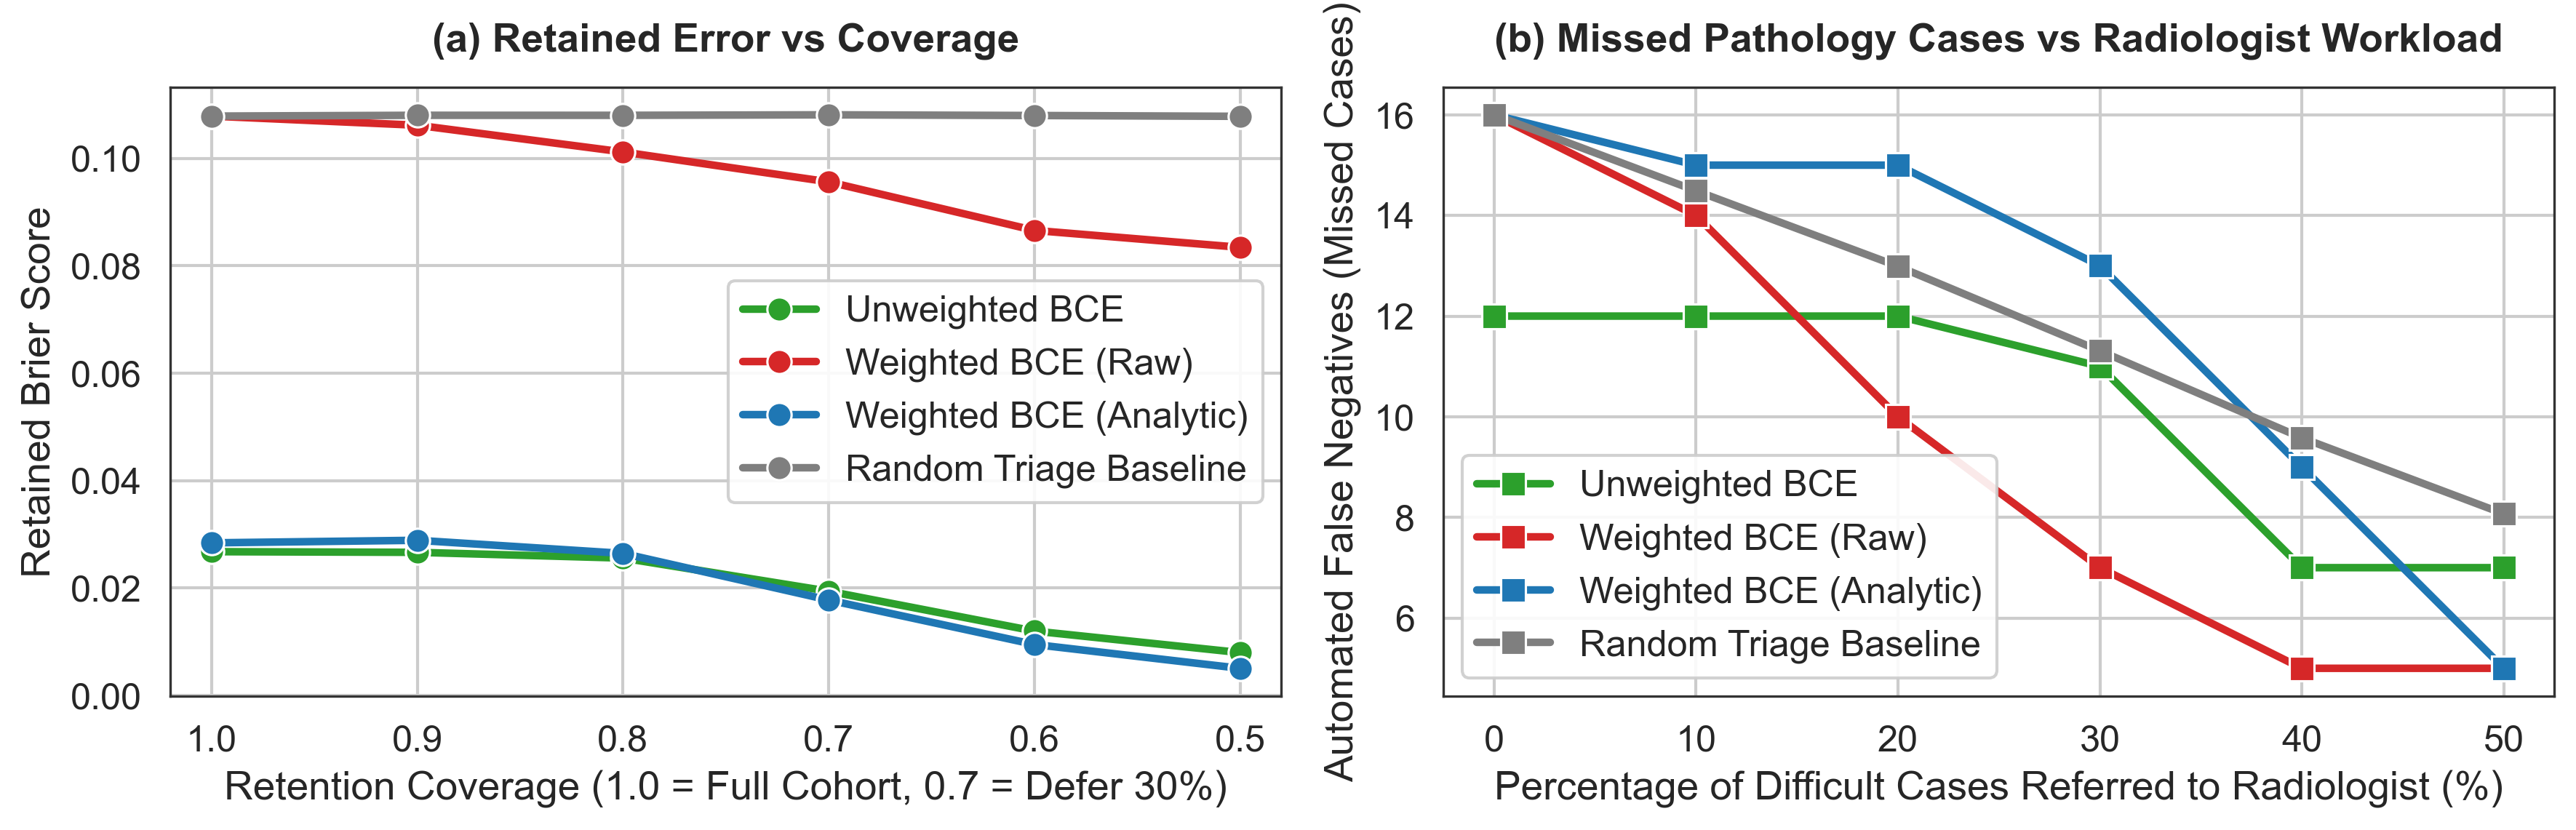
\includegraphics[width=0.85\textwidth]{figures/fig4_selective_risk_coverage.png}
\caption{Selective prediction evaluation on later held-out stratum $T_3$ with matched development thresholds (Table~\ref{tab:selective_prediction}). Left: Risk-coverage curves demonstrating that selective deferral steadily reduces Brier error across all models as ambiguous cases are referred. Right: Reader referral workload vs. automated false negatives, illustrating the distinct operational behaviors of raw weighted models (halving missed cases to 7.0 under 30\% referral) and analytic corrected models (optimizing probability accuracy with Brier 0.0178).}
\label{fig:selective_prediction}
\end{figure*}

Under selective deferral at 70\% coverage (30\% referral workload, 730 radiographs referred): raw weighted models halve automated false negatives from 16.0 to 7.0 (retained sensitivity 89.39\%, full-cohort triage sensitivity 91.76\%), but leave probabilities uncalibrated (Brier 0.0956); conversely, analytic calibrated models achieve superior probability estimation (Brier 0.0178), but retain 13.0 automated false negatives because threshold-distance normalization ($t^* \approx 0.022$) classifies low-probability false negatives ($\hat{p} \ll t^*$) as confident negatives. This reveals a fundamental operational trade-off: probability calibration is required for valid risk scoring, whereas raw weighted models with threshold-proximity triage act as a heuristic for recall-oriented screening. Neither system eliminates missed disease entirely.

\subsection{Cross-Institutional External Evaluation (MIMIC-CXR-JPG)}
The external MIMIC-CXR-JPG cohort comprised 3,403 frontal radiographs from 3,041 studies and 289 patients. Rather than asserting turnkey diagnostic transportability—given moderate discrimination for Pleural Effusion (AUROC $0.688$ [95\% CI: $0.656, 0.717$] DenseNet-121; $0.677$ ResNet-50), weak discrimination for Pneumonia ($0.583$--$0.607$) and Edema ($0.516$--$0.581$), and near-chance discrimination for Cardiomegaly ($0.519$--$0.525$)—this experiment functions as an external stress-test of zero-retraining recalibration under domain shift. Negative Brier skill scores ($\text{BSS} < 0$; Table~\ref{tab:mimic_external_validation}) confirmed substantial cross-institutional baseline calibration shift relative to a local null model ($\text{Brier}_{\text{null}} = \pi(1-\pi)$).

Paired analytic recalibration ($\bar{p}_{\text{corr}} = \frac{1}{3}\sum \sigma(z_s - \ln w)$) demonstrated statistically significant Brier reductions for Cardiomegaly ($\Delta\text{Brier} = -0.0579$ [95\% CI: $-0.0790, -0.0349$] DenseNet; $-0.0611$ [$-0.0818, -0.0415$] ResNet) and Pneumonia ($\Delta\text{Brier} = -0.0095$ [$-0.0170, -0.0016$] DenseNet; $-0.0155$ [$-0.0254, -0.0059$] ResNet), with point-estimate reductions on Pleural Effusion ($-0.0084$ and $-0.0109$). For Edema, subtracting theoretical $\ln w$ worsened Brier score (+0.0217), consistent with over-correction when empirical finite-network shifts saturate below theoretical $\ln w$. Diagnostic study-level sensitivity analysis ($N = 3,041$ studies across 289 patients, maximum probability pooling; Supplementary Table~S2) demonstrated identical concordance, confirming that recalibration patterns hold across radiographs and studies.

\begin{table*}[!t]
\caption{Cross-Institutional External Validation on the Official MIMIC-CXR-JPG Frontal Test Cohort ($N = 3,403$ Images from $3,041$ Studies Across $N = 289$ Unique Patients). Primary experimental evaluation of paired zero-parameter analytic logit recalibration ($\bar{p}_{\text{raw}} = \frac{1}{3}\sum \sigma(z_s) \to \bar{p}_{\text{corr}} = \frac{1}{3}\sum \sigma(z_s - \log w)$) on 3-seed ensembles trained with positive-weighted BCE. Evaluated with empirical prevalence ($\pi$), local null reference baseline ($\text{Brier}_{\text{null}} = \pi(1-\pi)$), patient-clustered 1,000-replicate bootstrap 95\% confidence intervals, Brier skill score ($\text{BSS} = 1 - \text{Brier}/\text{Brier}_{\text{null}}$), and paired contrast ($\Delta\text{Brier} = \text{Brier}_{\text{corr}} - \text{Brier}_{\text{raw}}$). The complete 16-row factorial comparison with unweighted BCE baselines is detailed in Supplementary Table~S1, and study-level sensitivity analysis is detailed in Supplementary Table~S2.}
\label{tab:mimic_external_validation}
\centering
\small
\resizebox{\textwidth}{!}{%
\begin{tabular}{llccccccc}
\toprule
\textbf{Architecture} & \textbf{Pathology} & \textbf{Prevalence ($\pi$)} & \textbf{$\text{Brier}_{\text{null}}$} & \textbf{AUROC [95\% CI]} & \textbf{Brier (Raw $\to$ Corr)} & \textbf{$\Delta\text{Brier}$ [95\% CI]} & \textbf{$\text{BSS}$ (Raw $\to$ Corr)} \\
\midrule
DenseNet-121 & Pleural Effusion & 32.18\% & 0.2182 & 0.668 [0.636, 0.700] & 0.2536 $\to$ 0.2451 & -0.0084 [-0.0401, +0.0240] & -0.162 $\to$ -0.123 \\
DenseNet-121 & Cardiomegaly & 26.33\% & 0.1940 & 0.525 [0.492, 0.558] & 0.2907 $\to$ 0.2328 & \textbf{-0.0579} [-0.0790, -0.0349] & -0.499 $\to$ -0.200 \\
DenseNet-121 & Pneumonia & 10.05\% & 0.0904 & 0.598 [0.553, 0.639] & 0.1078 $\to$ 0.0983 & \textbf{-0.0095} [-0.0170, -0.0016] & -0.192 $\to$ -0.087 \\
DenseNet-121 & Edema & 21.33\% & 0.1678 & 0.581 [0.549, 0.611] & 0.1914 $\to$ 0.2131 & +0.0217 [+0.0118, +0.0307] & -0.141 $\to$ -0.270 \\
\midrule
ResNet-50 & Pleural Effusion & 32.18\% & 0.2182 & 0.620 [0.588, 0.653] & 0.2665 $\to$ 0.2557 & -0.0109 [-0.0417, +0.0253] & -0.221 $\to$ -0.172 \\
ResNet-50 & Cardiomegaly & 26.33\% & 0.1940 & 0.522 [0.491, 0.552] & 0.2822 $\to$ 0.2211 & \textbf{-0.0611} [-0.0818, -0.0415] & -0.455 $\to$ -0.140 \\
ResNet-50 & Pneumonia & 10.05\% & 0.0904 & 0.589 [0.545, 0.629] & 0.1137 $\to$ 0.0982 & \textbf{-0.0155} [-0.0254, -0.0059] & -0.257 $\to$ -0.086 \\
ResNet-50 & Edema & 21.33\% & 0.1678 & 0.570 [0.538, 0.602] & 0.1929 $\to$ 0.2130 & +0.0201 [+0.0092, +0.0313] & -0.149 $\to$ -0.269 \\
\bottomrule
\end{tabular}%
}
\end{table*}

\section{Discussion}

\subsection{Decoupling Loss Distortion from Deidentified-Date Cohort Shift}
Our findings clarify the mechanism behind reported ``temporal calibration decay'' in medical AI~\cite{guo2022evaluation, hinson2022multisite}. While moderate discriminatory attenuation does occur across subsequent cohort strata (AUROC drops by $\approx 0.06$ identically across unweighted and weighted models), the perception of progressive calibration collapse is largely an artifact of positive loss weighting interacting with shifting disease prevalence. Because standard post-hoc evaluation relies almost exclusively on temperature scaling---which modifies logit dispersion without shifting the intercept---evaluators have routinely conflated static objective-loss bias with intrinsic temporal feature drift. When the mathematical logit offset is neutralized ($z - \ln w$), the apparent calibration collapse vanishes, and Brier scores track the unweighted baseline across all held-out strata.

\subsection{Relationship to Prior Theoretical and Clinical Literature}
Our theoretical framing connects with the work of Caplin, Martin, and Marx~\cite{caplin2022calibrating}, who demonstrated that class weighting corrupts calibration and derived an inverse likelihood recovery framework on static single-split tasks. We advance this literature into longitudinal clinical deployment: (i) resolving the temporal calibration decay paradox across sequential deidentified-date cohort strata; (ii) proving the structural failure of temperature scaling ($\alpha \approx -2.96$); (iii) demonstrating finite-network optimization bounds ($w > 1000$ in Edema saturates at $\Delta z \approx 3.69$ vs. theoretical $7.00$); and (iv) stress-testing cross-institutional transfer from BRAX to MIMIC-CXR. Furthermore, extending multi-dataset selective CXR investigations~\cite{aperstein2026knowing}, we operationalize the clinical triage trade-off: analytic offset ($z - \ln w$) is essential for epidemiological risk stratification and prognosis (restoring Brier parity, consistent with plug-in principles~\cite{piccininni2024understanding}), while raw weighted models support recall-oriented screening triage under referral budgets.

\subsection{Architectural Universality and Operational Utility}
The observed phenomena are consistent across architectures: DenseNet-121 and ResNet-50 exhibit identical discrimination attenuation ($\Delta\text{AUROC} = -0.0604$ vs. $-0.0687$), severe raw calibration intercepts ($\alpha \approx -2.96$ and $-2.85$), and comparable Brier reductions under Analytic Offset ($73.7\%$ and $76.3\%$, $\Delta\text{Brier} = -0.0795$ and $-0.0936$). Because Analytic Offset ($z - \ln w$) operates in constant time ($O(1)$) with zero validation fitting and zero refitting, it provides an immediate algorithmic solution for resource-constrained edge devices and PACS pipelines.

\subsection{Scope, Boundaries, and Methodological Limitations}
Several methodological limitations define the boundary of these findings:
\begin{enumerate}
    \item \textbf{Date Anonymization and Temporal Semantics:} In BRAX, dates are fictitious hashes preserving intra-patient acquisition intervals; cross-patient calendar synchronization is unverified. Partitions ($T_1, T_2, T_3$) reflect sequential deidentified-date strata rather than synchronized calendar years.
    \item \textbf{Cross-Institutional Domain Gap and Modest Transportability:} External validation on MIMIC-CXR-JPG yielded modest discrimination (Effusion AUROC $\approx 0.69$) and near-chance discrimination for Cardiomegaly ($0.52$). While analytic offset reduced Brier error for Cardiomegaly and Pneumonia, it worsened Edema ($+0.0217$), demonstrating that zero-retraining offset correction cannot compensate for severe cross-institutional covariate shift or negative transfer.
    \item \textbf{Label Extraction Noise and Retrospective Simulation:} Labels were derived from Portuguese reports via NLP rather than multi-radiologist panel review, and evaluations were retrospective. Real-world validation requires prospective silent shadow deployment in operational hospital PACS.
    \item \textbf{Architectural Scope and Scarcity Bounds:} We evaluated standard CNN backbones (DenseNet-121, ResNet-50); Vision Transformers and vision-language models warrant future investigation. Under extreme class scarcity (Edema, $w = 1091.3$), empirical logit shifts saturate at $+3.69$ due to $L_2$ regularization, defining the empirical boundary of the asymptotic derivation.
\end{enumerate}

\section{Conclusion}
In this controlled study across 40,523 BRAX radiographs, severe probability miscalibration across held-out strata was predominantly driven by positive loss weighting rather than progressive temporal drift. Because standard temperature scaling cannot shift the logit intercept, it leaves this distortion intact. A constant-time closed-form analytic offset ($z - \ln w$) eliminates 73.7\% of stratum $T_3$ Brier error ($0.1079 \to 0.0284$, $\Delta\text{Brier} = -0.0795$ [95\% CI: $-0.0893, -0.0697$]) without model refitting or validation data, restoring calibration parity with unweighted models. Furthermore, selective triage simulations reveal an operational trade-off: raw weighted models provide effective recall-oriented triage by halving missed cases under a 30\% referral budget, whereas analytic calibration restores reliable probabilities for decision-theoretic risk stratification. Neither approach eliminates missed disease entirely, underscoring the necessity of transparent, workload-aware deployment policies in clinical deep learning.

\section*{CRediT Authorship Contribution Statement}
\textbf{Vishesh Panghal}: Conceptualization, Methodology, Software, Validation, Formal Analysis, Investigation, Data Curation, Writing -- Original Draft, Writing -- Review \& Editing, Visualization, Project Administration.

\section*{Declaration of Competing Interest}
The author declares that he has no known competing financial interests or personal relationships that could have appeared to influence the work reported in this paper.

\section*{Data and Code Availability}
The BRAX dataset (v1.1.0)~\cite{reis2022brax} is available on PhysioNet at \url{https://physionet.org/content/brax/1.1.0/} under the PhysioNet Credentialed Data Use Agreement. The MIMIC-CXR-JPG database (v2.1.0)~\cite{johnson2019mimic,johnson2019mimicjpg} is available on PhysioNet at \url{https://physionet.org/content/mimic-cxr-jpg/2.1.0/} under the PhysioNet Credentialed Data Use Agreement. Access requires credentialed PhysioNet researcher status, completion of human subjects research training, and signed data use agreements. Complete end-to-end replication scripts, model evaluation routines, cross-fitting recalibration pipelines, selective prediction triage simulations, and tabular evaluation artifacts are openly available on GitHub at \url{https://github.com/Vishesh-panghal/temporal-brax-calibration}, and the repository will be permanently assigned a persistent DOI via Zenodo upon acceptance of the manuscript. No credentialed patient-level images, metadata, labels, identifiers, or prediction rows are redistributed; the repository contains aggregate evaluation artifacts and a synthetic manifest schema example.

\section*{Ethical Approval and Consent to Participate}
This study represents a secondary analysis of credentialed-access, de-identified diagnostic imaging databases accessible under formal Data Use Agreements. The primary BRAX dataset collection was approved by the Institutional Review Board (IRB) of Hospital Israelita Albert Einstein (S\~ao Paulo, Brazil; CAAE: 36720520.1.0000.0071) with a formal waiver of informed consent. Creation and distribution of the MIMIC-CXR-JPG database was approved by the Institutional Review Boards of Beth Israel Deaconess Medical Center (Boston, MA) and the Massachusetts Institute of Technology (Protocol \#0403000206) with a waiver of informed consent. The author completed mandatory human subjects research training (CITI Program certification), executed approved PhysioNet Data Use Agreements for both databases, and strictly complied with data governance protocols prohibiting re-identification or redistribution of protected health information.

\section*{Declaration of Generative AI and AI-Assisted Technologies in the Writing Process}
During the preparation of this work, the author utilized generative artificial intelligence platforms (Google Gemini, Anthropic Claude, and OpenAI Codex) exclusively for LaTeX formatting and syntax verification, analysis code refactoring and modularization, grammatical refinement, and bibliographic cross-referencing. Following the use of these tools, the author thoroughly reviewed, verified, and edited all text, numerical outputs, and code, and takes full intellectual and scientific responsibility for the integrity, validity, and conclusions of the published manuscript.

\section*{Funding}
This research did not receive any specific grant from funding agencies in the public, commercial, or not-for-profit sectors.

\bibliographystyle{elsarticle-num}
\bibliography{references}

\end{document}
